\section{Lucky Patcher} \label{section:luckypatcher-explain}
On the official website, Lucky Patcher is described as "[...] a great Android tool to remove ads, modify apps permissions, backup and restore apps, bypass premium applications license verification, and more" \cite{luckyPatcherOfficial}.
It is written by a developer called ChelpuS and currently on version is 6.0.4 (on 02/17/2016).
\newline
Lucky Patcher offers different patches.
They include the removing of the license verification premium apps to crack their \gls{drm}, removing of Google Ads, changing and restricting of permissions and activities as well as creation modified after applying one of the feature above on the original \gls{apk}s \cite{luckyPatcherOfficial}.
Since copy protection by Google is deprecated, all applications are stored in \textit{/data/app/}.
The user as well as \gls{luckypatcherg} can access this folder and copy applications from it.
\textit{Root} and busybox, an application which provides standard UNIX tools for Android\cite{busyboxApp}, is only required when the application should be modified on the device, which is explained later.
\gls{luckypatcherg} requires no technical knowledge and offers automatic cracking for non professionals.
This combination makes it a popular and an effective tool with a high damage potential. \cite{munteanLicense}
\newline
This thesis focuses on how Lucky Patcher is bypassing the license verification mechanism of applications.
The goal of circumventing the license check is to make the pirated application work as if had been legally acquired in the store.
As described in section~\ref{section:lvl}, the license verification is implemented as client-server connection.
The app sends information about the user and the application to the server, which checks and verifies the given information, and replies with an approval or rejection.
The server communication is secure against man in the middle attacks or spoofing, as messages are private key encrypted \cite{munteanLicense}.
\gls{luckypatcherg} is taking a different path by modifying the application itself. This will be analysed in detail in the following chapters after explaining the general usage.
\newline
\begin{figure}[h]
    \centering
    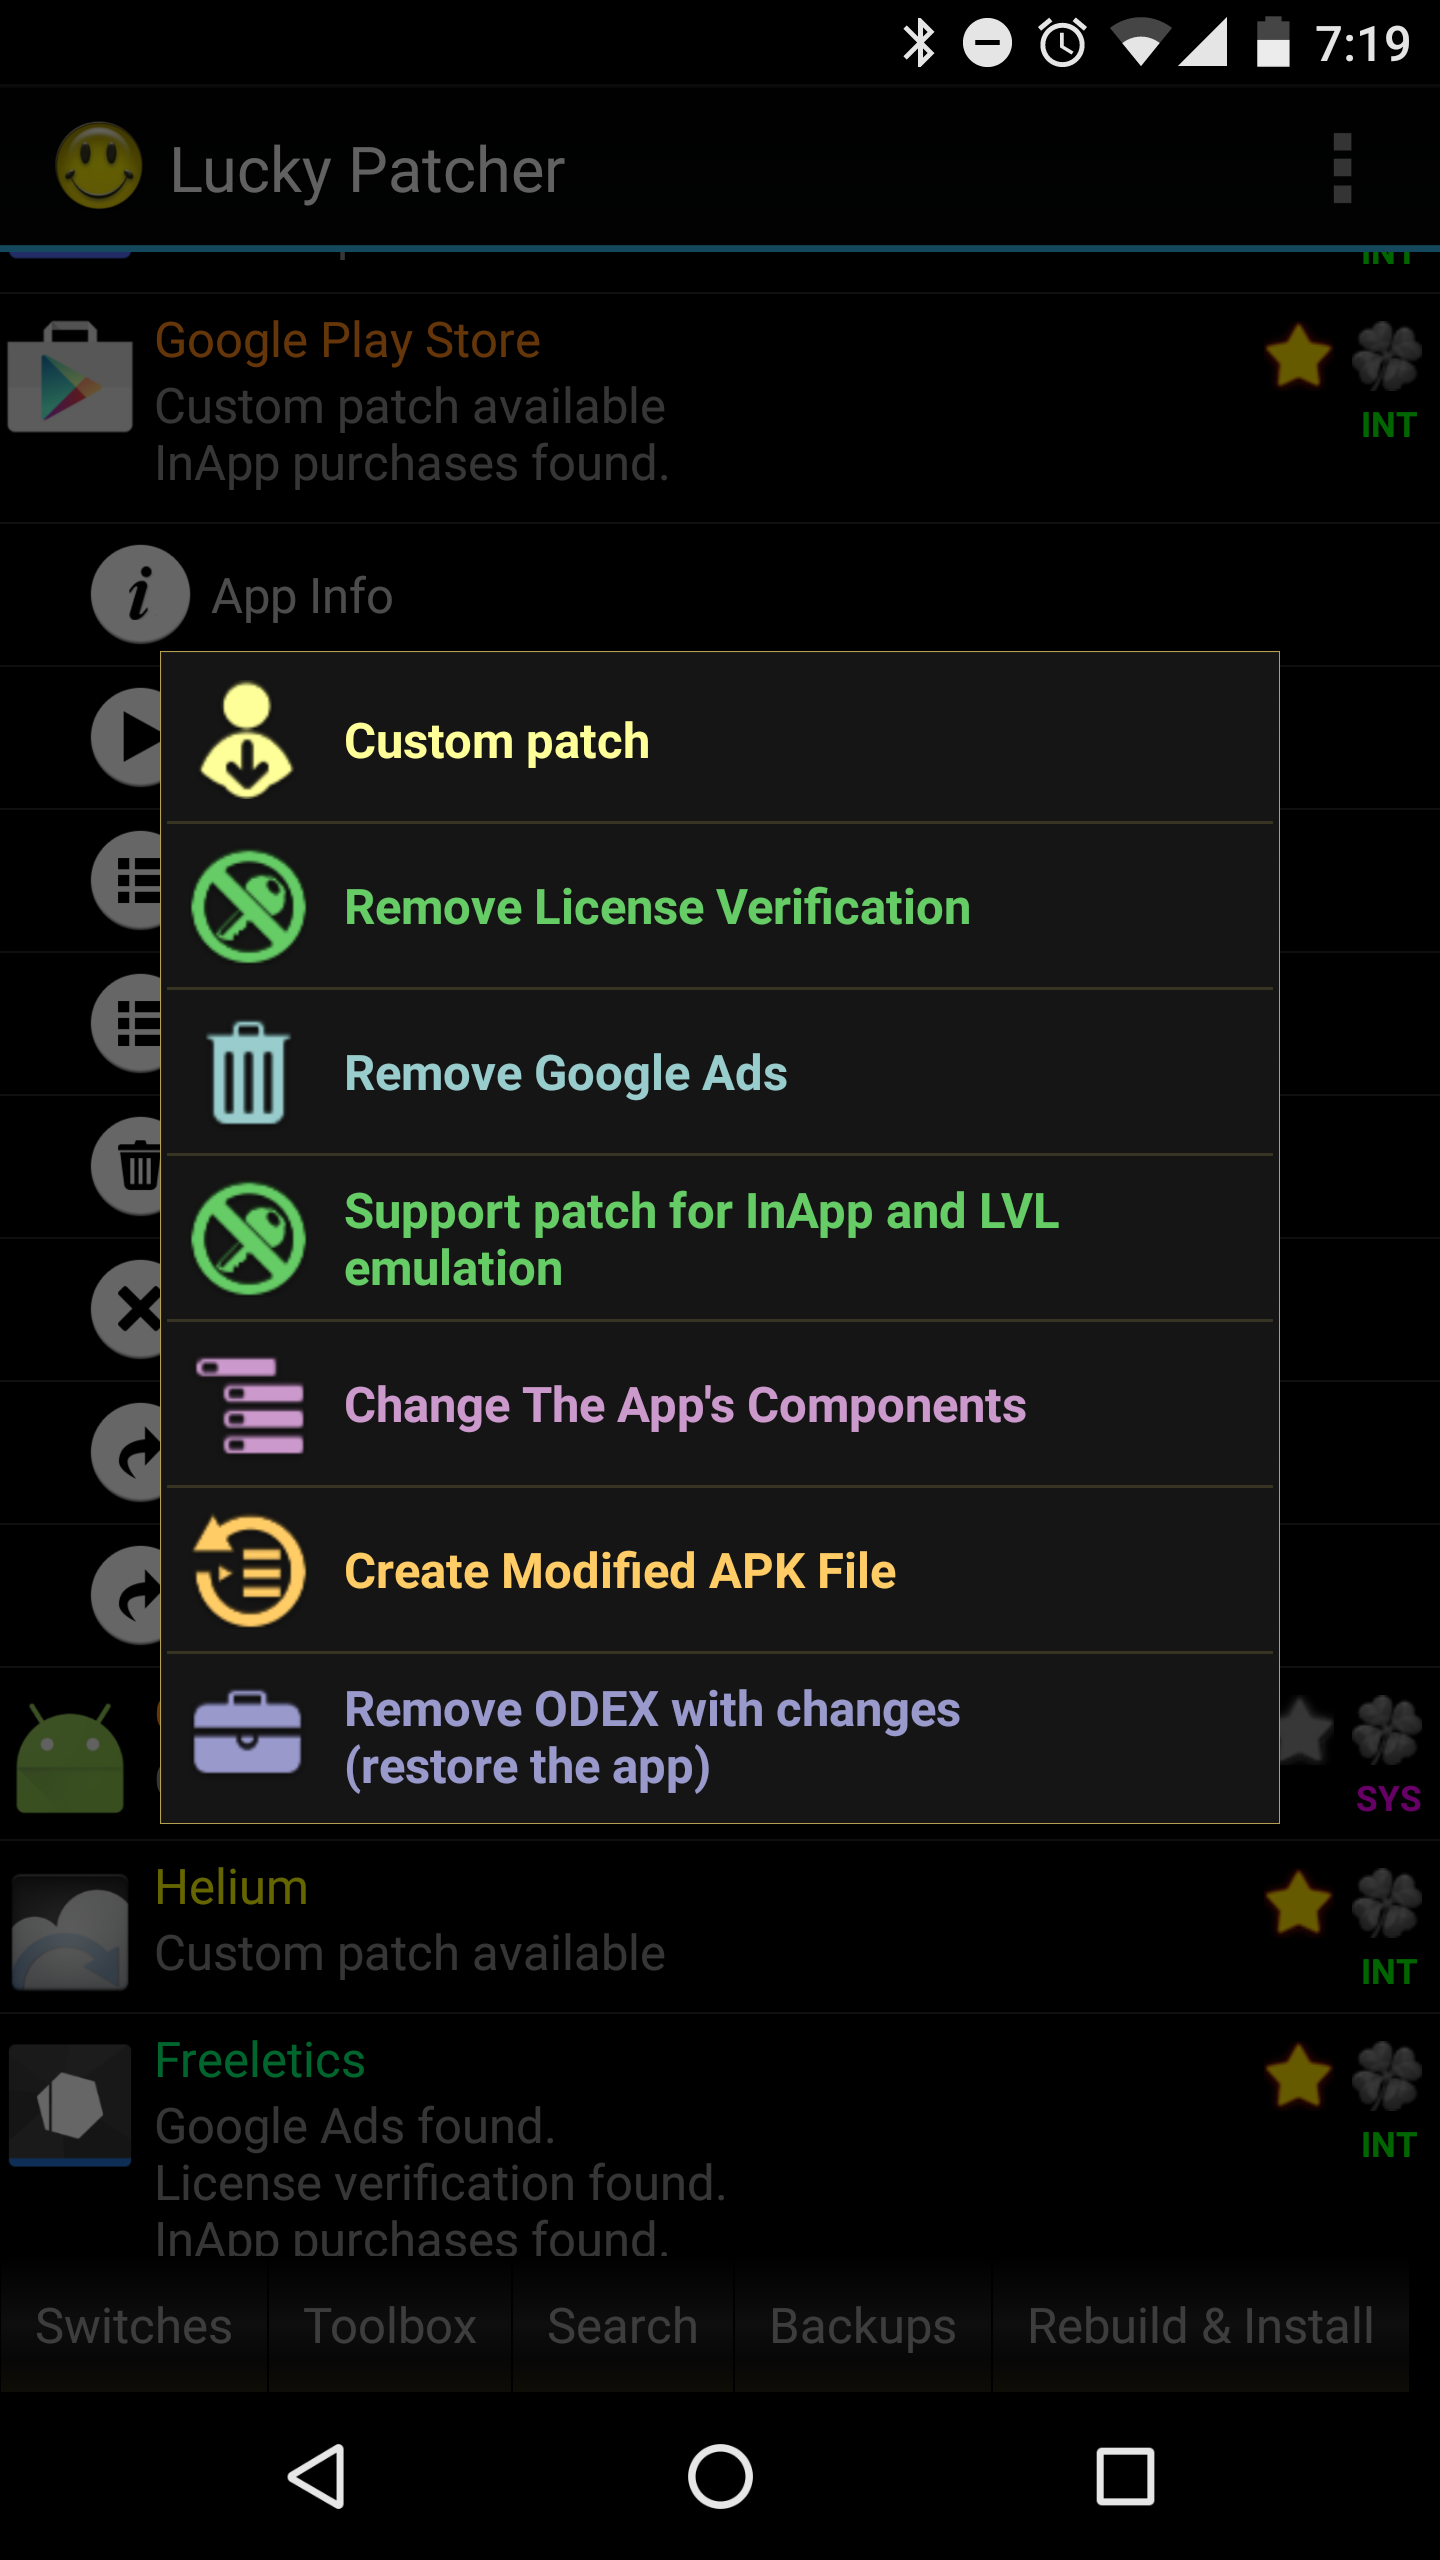
\includegraphics[width=0.3\textwidth]{data/luckyFeatures.png}
    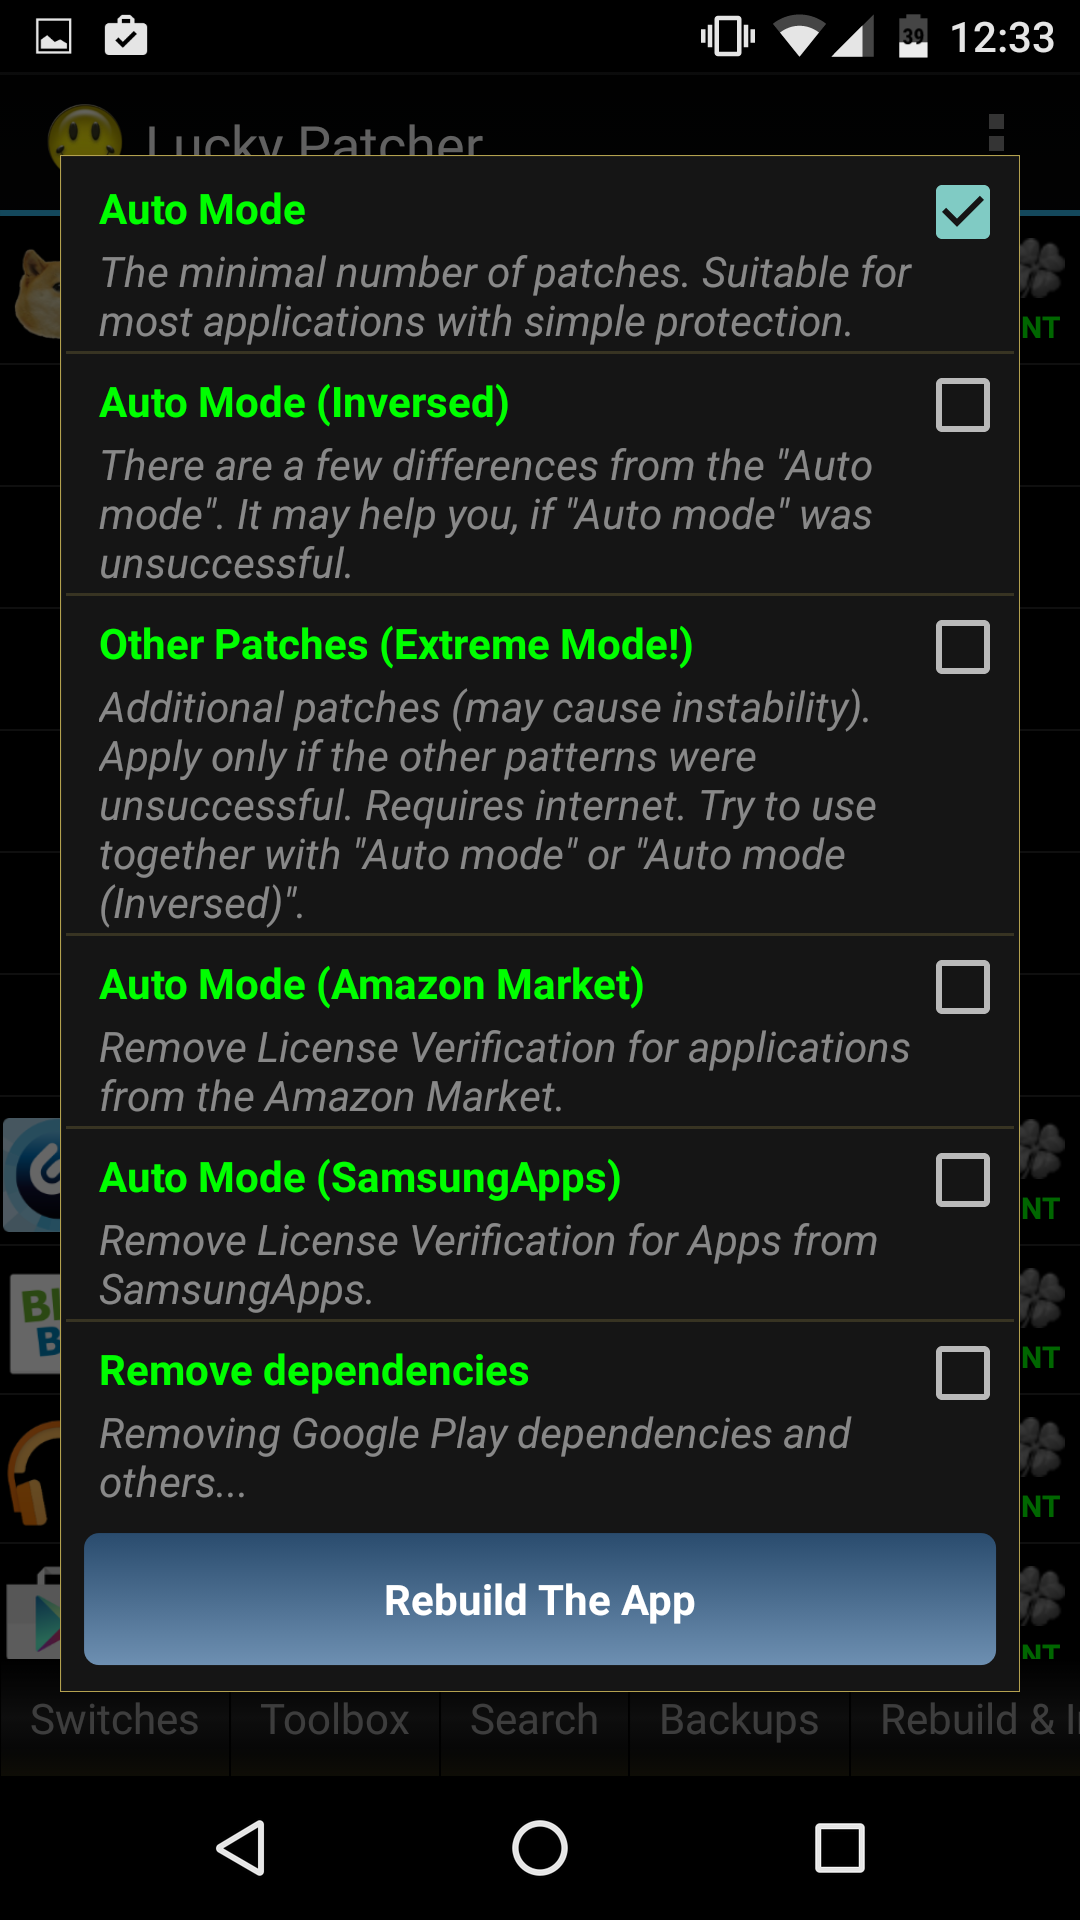
\includegraphics[width=0.3\textwidth]{data/luckyModi.png}
    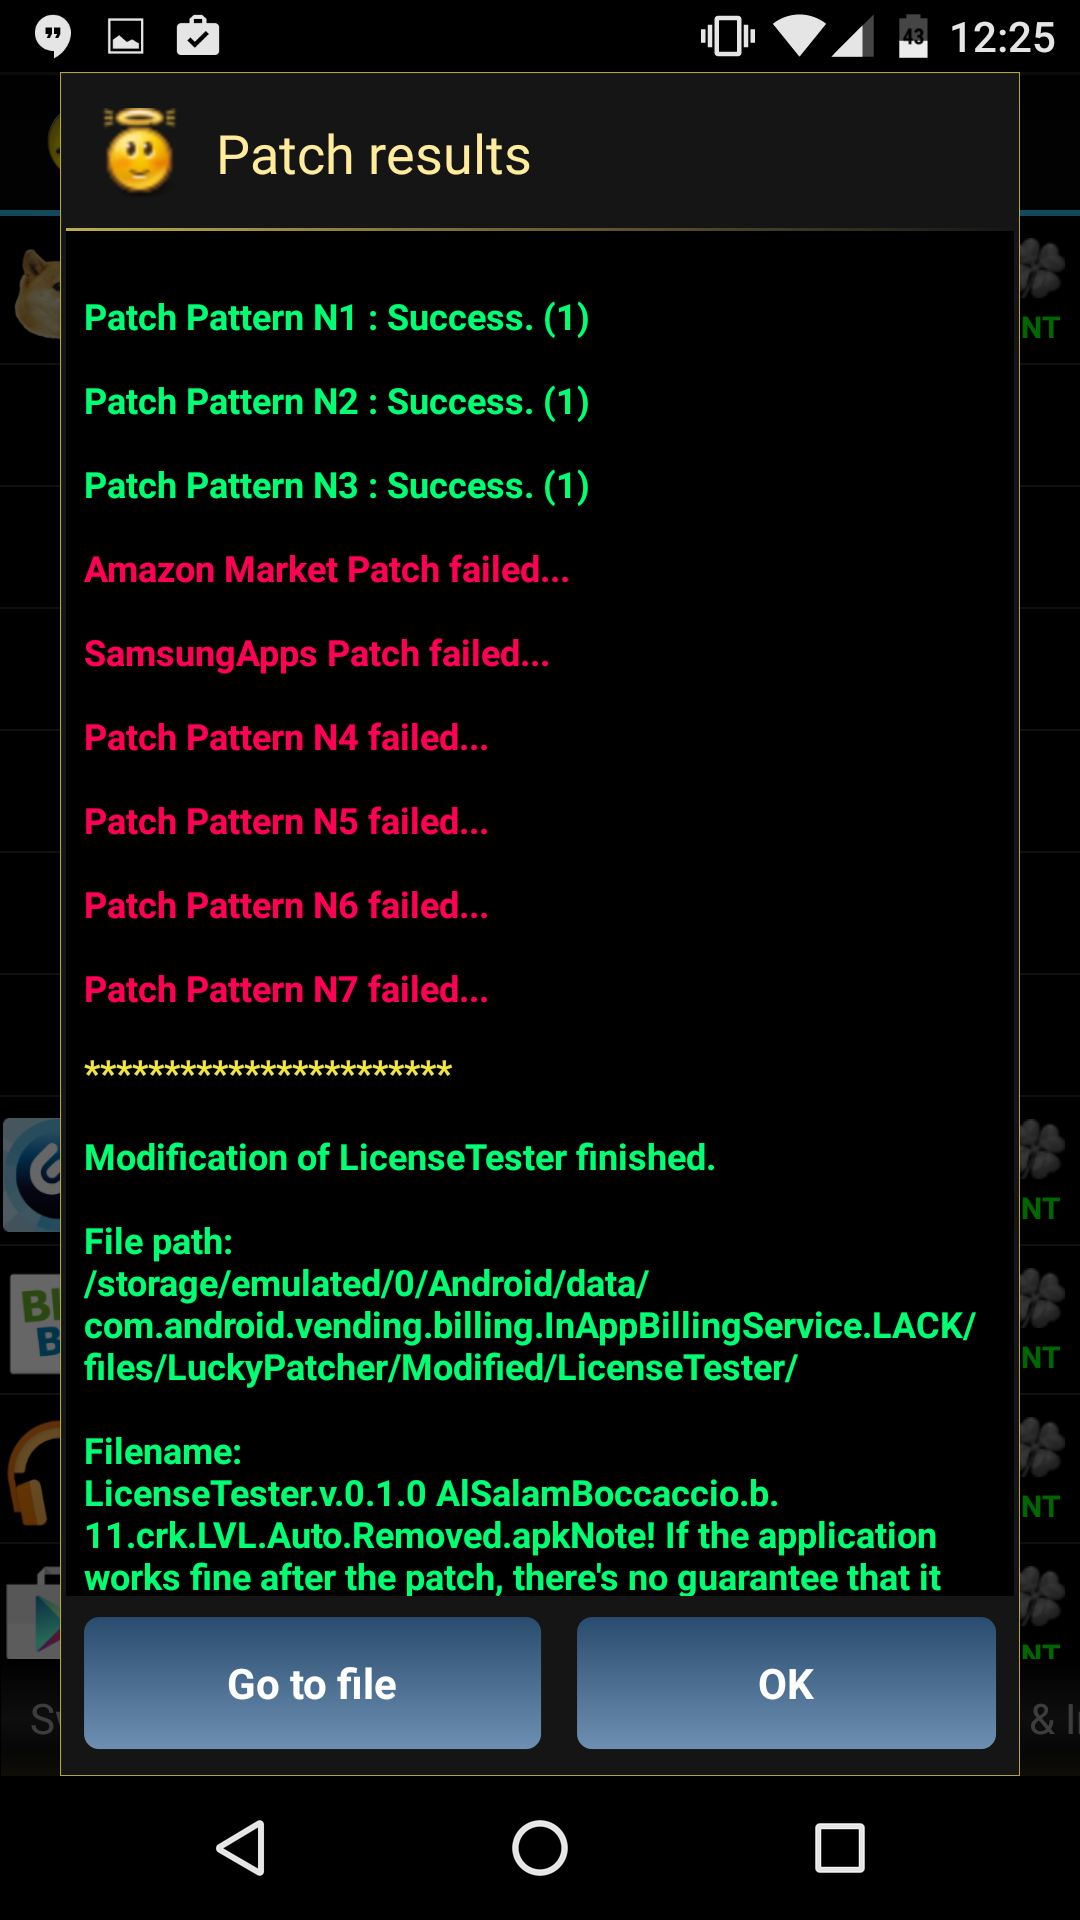
\includegraphics[width=0.3\textwidth]{data/luckyPatching.png}
    \caption{Left to right: Features offered LuckyPatcher, modes to crack license verification and the result after patching}
    \label{fig:luckyScreen}
\end{figure}

Using Lucky Patcher is fairly simple.
The application can be downloaded from the official website \cite{luckyPatcherOfficial} as an \gls{apk} and installed on the device.
In order to have the features available, the device has to be rooted.
On startup of \gls{luckypatcherg}, all installed applications are shown in a list.
A colored text about what patches can be applied is shown below each name.
When an application is selected, a submenu offers various actions, e.g. to get information about the app or run it.
\newline
\newline
When the patches menu is selected, the submenu of figure~\ref{fig:luckyScreen}, on the left, is shown.
It shows the available patches for this application.
There are two types of patches.
The first type is the \textit{custom patch} and the second type are universal patches.
They can be used for the disabling of the license verification libraries, removing Google Ads and rebuilding of the application to use the emulated \gls{lvl} and in-app billing \gls{api}.
\newline
\gls{luckypatcherg} offers two different approaches to apply these patches.
The first approach is directly on the device and requires \textit{root}.
This method creates an \gls{odex} in the Dalvik cache on the phone.
The second approach is the creation of a modified \gls{apk}.
When selected, this approach offers the same patches as the first one but they are not applied directly on the phone.
This approach copies the application of choice from the storage, applies the desired patch and creates a new \gls{apk}.
This cracked application can either be distributed to other devices or installed on the device after removing the original \gls{apk}.
\newline
The custom patch is the most powerful modification.
It applies application specific changes.
They have to be provided by users who reverse engineered the specific application and created a solution tailored for the application.
The patches are either already cracked native libraries, replacing the provided \textit{*.so} file, or a bytecode sequence injected into the application, disabling the desired feature.
\newline
This thesis focuses on the \textit{Auto Modes} for the license verification.
There are six automatic modes available as seen in figure~\ref{fig:luckyScreen} in the middle.
Their description is rather short and does not offer information of how the modes are working.
\newline
When a mode is chosen and the patching is finished, a result overview is shown.
As seen in figure~\ref{fig:luckyScreen} on the right, different patching patterns are used to remove license verification.
The different patching patterns are analysed and explained in section~\ref{section:luckypatcher-patterns}.
Lucky Patcher does guarantee that the result is working and all license verification related restrictions are removed.
\newline
In this thesis, Lucky Patcher is analysed in two different ways.
\begin{itemize}
\item inspection of the source code
\item blackbox analysis using cracked applications
\end{itemize}
